%--------------------------------------------------------------------------------------------------------------
% kapitel/grundlagen.tex
%--------------------------------------------------------------------------------------------------------------

\chapter{Theoretische Grundlagen}

In diesem Kapitel werden zunächst die Grundlagen und Begrifflichkeiten vorgestellt. Weiterhin werden die Kriterien für eine erfolgreiche Migrationen erläutert.

\section{SIV.\@AG}\label{SIV.AG}

Die SIV.\@AG ist ein Anbieter für ganzheitliche Lösungen im Bereich der deutschen und internationalen Energie- und Wasserwirtschaft. Das Kernstück des Unternehmens ist das Softwareprodukt kVASy$^\text{\textregistered}$, ein vollständig integriertes \acrfull{erp}-System, welches insbesondere auf die Anforderungen und Prozesse der Energie- und Wasserwirtschaft ausgerichtet ist. Das Unternehmen wurde 1990 durch Jörg Sinnig als Software- und Beratungshaus gegründet und im Februar 2016 an die Harris Computer Corporation, einer Tochtergesellschaft der Constellation Software Inc. verkauft. Zum gegenwärtigen Zeitpunkt beschäftigt die SIV.\@AG mehr als 400 Mitarbeiter. Ihr Leistungsportfolio reicht von der Beratung und Analyse über die Implementierung und Bereitstellung der IT-Systeme bis hin zur Datenmigration, Schulung und Pflege. \cite{SIV13}

\section{kVASy$^\text{\textregistered}$}\label{kvasy} 

Das zuvor bereits erwähnte kVASy$^\text{\textregistered}$ ist ein webbasiertes \acrshort{erp}-System und bildet das Aushängeschild der SIV.\@AG. Unter einem \acrshort{erp}-System ist eine integrierte unternehmensweite Anwendung zu verstehen, die zur Koordination wichtiger interner Prozesse eingesetzt wird \cite[Seite 482]{kjd2010}. Zu der Produktfamilie von kVASy$^\text{\textregistered}$ gehören die Module Finance (Buchhaltung), Billing (Abrechnung) und EDM (Vertragsverwaltung), Technical Assets (Anlagenmanagement) und xRM (Kundenbeziehungsmanagement) (vgl. Bild \ref{pic:kVASy:end}).
\begin{figure}[ht]
	\begin{center}
		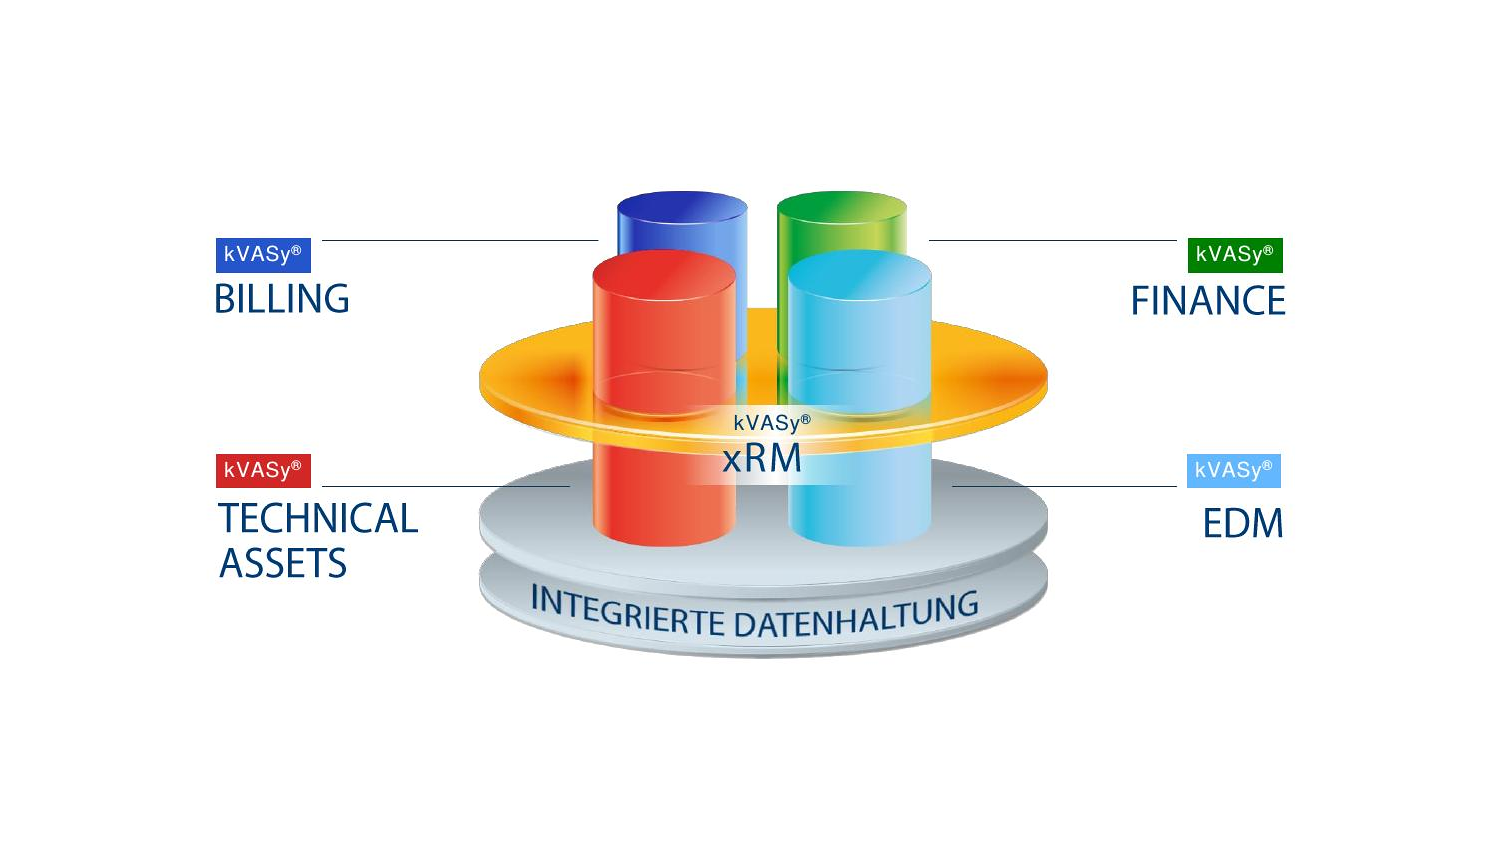
\includegraphics[scale=0.25]{bilder/kVASy_Schema.png}
		\caption{Produktfamilie von kVASy$^\text{\textregistered}$\cite{SIV16}}
		\label{pic:kVASy:end}
	\end{center}
\end{figure}
Auf der Grundlage einer zentralen Datenbasis erfolgt die Kommunikation der Module und Funktionalitäten schnittstellenfrei \cite[Seite15]{SIV13}. Die Umsetzung dessen erfolgt durch das \acrfull{dbms} Database 11g Release 2 von der Firma Oracle. Für die Umsetzung der Applikationslogik wurde \acrfull{plsql} verwendet, eine proprietäre Programmiersprache der Firma Oracle \cite{wiki:plsql}.

\section{Datenbankgrundlagen} 
Indirekt wird bei Datenbanken von dem weit verbreiteten \acrfull{rdbms} ausgegangen. Dieses Datenbankmodell ist eins der Populärsten \acrshort{rdbms} \cite{DB16}.  Ein Datenbanksytem besteht Zu den Aufgaben eines Datenbanksystems gehört es die Daten möglichst effizient und dauerhaft zu speichern. Zudem soll es eine Vereinfachung der Datenverwaltung ermöglichen. Das relationale Datenmodell ist so konzipiert das es eine mengenorientierte Datenverarbeitung erlaubt. Dabei können die Daten aus mehreren Tabellen durch Join-Verknüpfungen in einer großen Tabelle abgebildet werden. Durch die Festlegung von Spalten und Where-Klauseln kann die Menge weiter bearbeitet und somit in der Höhe und Breite eingeschränkt werden. Im Gegensatz zu einem datensatzorientiertem Vorgehen wird die Tabelle, Zeile um Zeile abgerufen und nach bestimmten Kriterien geprüft. Nachdem die Kriterien erfüllt sind werden die Daten weiterverarbeitet. \cite{Kemper2011}[Seite 71] Somit wird die mengenorientierte Datenverarbeitung durch die Datenbanksprache SQL ausgeführt und die datensatzorientierte Verarbeitung beispielsweise durch eine Programmiersprache C\texttt{++} oder Java. Die relationale Datenbank von Oracle die in der Bachelorarbeit verwendet wird, bietet die Möglichkeit eine Programmiersprache, wie etwa \acrshort{plsql} die eigens von Oracle entwickelt worden ist einzusetzen. Durch \acrshort{plsql} ist es somit Möglich Java-Programme oder C\texttt{++}\,-Programme in einem \acrshort{plsql}-Programm auszuführen.

\subsection{Elemente einer relationalen Datenbank}
Zu den Elementen gehören Tabellen, Spalten und Zeilen (auch Tupel genannt). In der Regel besteht eine Datenbank aus mindestens einer, meistens aber aus mehreren \textbf{Tabellen} (Relationen). Die wiederum Attribute oder auch Felder beinhalten, die sogenannten Spalten. Eine \textbf{Spalte} besitzt einen Namen sowie einen Datentyp. Zu den drei wesentlichen Datentypen zählen Number (Zahl), Varchar (Text) und Date (Datum), diese enthalten wiederum noch weitere Varianten \cite{Kemper2011}[Seite 112]. Die Bedeutung eines Datentyps ist zum einen für ein Datenbanksystem, sowie für den Anwender wichtig. Bei einem Datenbanksystem ist eine Optimierung des physikalischen Datenspeichers möglich. Beim Anwender dient der Datentypen zur Überprüfung der Eingabe, die er getätigt hat. Sollte der vorgegeben Datentyp dem nicht Entsprechen würde es in so einem Fall zu einer Fehlerausgabe führen. Damit kann der Anwender darauf reagieren und die Eingabe korrigieren.
Die \textbf{Zeilen} (Tupel) bezeichnen die eigentlichen Datensätze. Eine Zeile beinhaltet für jede Spalte einen Wert. Sollte kein Wert angegeben sein wird die Spalte mit dem Wert NULL befüllt. NULL ist somit als Wert zusehen und steht nur für die Abwesenheit eines Wertes. Die Abbildung \ref{pic:RDB:end} zeigt noch einmal eine Tabelle mit den Begrifflichkeiten die im Bereich der relationalen Datenbanken zum Einsatz kommen.
\begin{figure}[ht]
	\begin{center}
		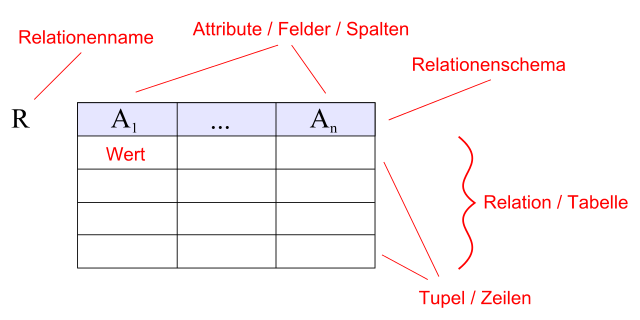
\includegraphics[scale=0.5]{bilder/Begriffe_relationaler_Datenbanken.png}
		\caption{Begriffe einer relationaler Datenbanken \cite{wiki:rdb}}
		\label{pic:RDB:end}
	\end{center}
\end{figure}

Zu den Vorteilen einer relationalen Datenbank gehören neben der Mehrbenutzerfähigkeit und Transaktionen auch Datensicherheit und Datenintegrität.
Eine Transaktion bezeichnet eine Folge von Datenverarbeitungsbefehlen (lesen, verändern, einfügen, löschen), welches den Datenbestand in einen konsistenten Zustand überführt. Eine Transaktion sollte daher entweder vollständig und fehlerfrei oder gar nicht ausgeführt werden. \cite{Kemper2011}[Seite 285] Zur Datensicherheit zählt sowohl der Schutz vor Datenverlust, als auch der unerlaubte Zugriff durch Dritte. Die Datenintegrität wird durch sogenannte Constraints erreicht. Sie definieren Bedingungen, die beim Einfügen, Ändern und Löschen von Datensätzen in der Datenbank erfüllt werden müssen. \cite{Kemper2011}[Seite 159-161]

\subsection{Beziehungen}
In einem relationalen Datenbanksystem werden die Beziehungen zwischen Daten, mit Hilfe von Schlüsselspalten realisiert.  
Diese Schlüsselspalten werden durch Constraints gebildet. Dazu gehören PRIMARY KEY, FOREIGN KEY und UNIQUE \cite{Kemper2011}[Seite 161]. Der PRIMARY KEY und der FOREIGN KEY sollen etwas näher erläutert werden. Der PRIMARY KEY bestimmt eine oder mehrere Spalten als Primärschlüssel. Die Werte dieser Schlüsselspalten sind immer eindeutig und dürfen nicht NULL sein. Zudem ist eine Primärschlüssel nur einmal für eine Tabelle definierbar. Der FOREIGN KEY dient als Verknüpfung zwischen Tabellen. Dafür wird der Primärschlüssel aus der ersten Tabelle in die zweite Tabelle als Fremdschlüssel eingetragen. Der Fremdschlüssel enthält somit den gleichen Wert wie der Primärschlüssel. Des Weiteren kann der Fremdschlüssel in einer Tabelle einmal, keinmal oder mehrmals vorkommen.

\subsection{Schema und Ausprägung}
Es gibt gewisse Unterschiede zwischen einem Datenbankschema und einer Datenbankausprägung. Das Datenbankschema beschreibt nicht die einzelnen Datenobjekte, sondern es legt die Struktur der abspeicherbaren Datenobjekte fest. Somit handelt es sich bei einem Datenbankschema um Daten, die andere Daten beschreiben diese können auch als Metadaten aufgefasst werden. Im Gegensatz dazu ist bei der Datenbankausprägung, die einem ständigen Wandel unterliegt, der gegenwärtig gespeicherte Zustand zu verstehen. Somit bildet das Datenbankschema die Basis der Datenbankausprägung. Die beiden Begriffe werden im Zusammenhang mit einer Datenbank auch als intensionalen (Schema) und extensionalen (Ausprägung) Ebene bezeichnet. Die Änderung eines Datenbankschemas wird normalerweise sehr selten vorgenommen, wenn dies doch passiert spricht man von einer \textit{Schemaevolution}. Zu Beachten ist dabei, dass eine Schemaänderung schwerwiegenden Folgen haben kann. Grund dafür ist das Aufweisen einer inkonsistenten Struktur der bereits abgespeicherten Datenobjekte. \cite{Kemper2011}[Seite 24]

\section{Datenintegration/Datenmigration}
Der Begriff Migration stammt von dem lateinischen Begriff migratio und bedeutet (Aus)wanderung, d.\,h. die Übernahme von
Daten in ein anderes System, um sie dort wieder im vollem Ausmaß zu nutzen \cite{duden:migra}.
Die Datenmigration oder auch Datenübernahmen genannt, verläuft von einem Quellsystem hinzu einem Zielsystem. Dabei beinhaltet das Quellsystem, die zu migrierenden Daten und das Zielsystem die importierten Daten. In dieser Arbeit wird das in Kapitel \ref{kvasy} auf Seite \pageref{kvasy} beschriebene kVASy$^\text{\textregistered}$, als Zielsystem verwendet.

\section{Transformationen}

\section{\acrshort{etl}-Prozess}
Die Abkürzung \acrshort{etl} setzt sich aus den drei Wörtern Extraktion, Transformation und Laden zusammen. Sie wird oft mit dem Begriff Data Warehouse in Zusammenhang gebracht. Dabei dient \acrshort{etl} dazu, unterschiedliche Bereiche Buchhaltung, Abrechnung, Vertragsverwaltung usw. in eine zentrale Datenbank (Data Warehouse) zusammenzuführen. Ziel ist es z.\,B. eine umfassende Sicht auf den Kunden zu bekommen. Aufbauend darauf können komplexe Analysen entwickelt werden, um eine erfolgreiche und wohl überlegte Geschäftsentscheidung zu treffen. Bei der Abfolge eines \acrshort{etl}-Prozesses werden zunächst Daten aus einer Datenquelle extrahiert. Daraufhin werden diese mit Hilfe von Transformationsregeln homogenisiert. Schließlich werden im letzten Schritt die angereicherten oder bereinigten Daten in das Ziel geladen. Die Bandbreite für den Einsatz eines \acrshort{etl}-Prozesses erstreckt sich über das Datenqualitätsmanagement sowie der Replikation und Synchronisation von Daten bis hin zu der Migration von Daten aus Altsystemen. Letzteres ist für die Bachelorarbeit der wichtigste Aspekt und wird dahin gehend genauer untersucht. \cite{Rossak2013}
\begin{figure}[ht]
	\begin{center}
		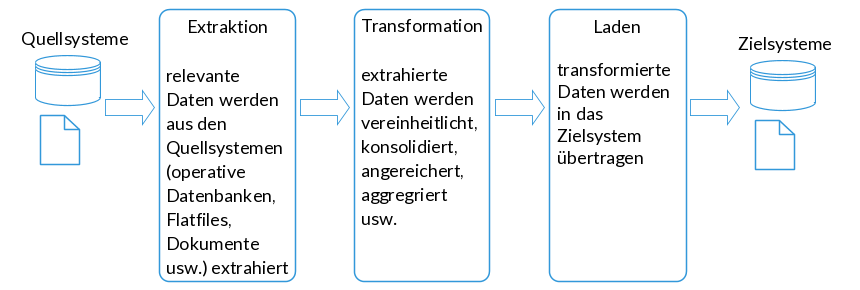
\includegraphics[scale=0.65]{bilder/ETL-Prozess.png}
		\caption{Allgemeiner ETL-Prozess (eig. Abb. nach \cite{Rossak2013}[Seite 38])}
		\label{pic:ETL:Pro}
	\end{center}
\end{figure}
\subsection{Extraktion}

\subsection{Transformation}
\subsection{Laden}
 

\section{Qualitätskontrolle/Protokollierung}

\section{Kriterien für eine Softwaremigration}
Ziel dieser Bachelor-Thesis ist es den Einsatz des ETL-Tools im Prozess der Datenmigration zu Untersuchen. Für eine Softwaremigration ist eine Vielzahl an Kriterien zu beachten. Diese allgemeinen Kriterien werden als Leitfaden für die Migration von Software durch die Beauftragte der Bundesregierung für Informationstechnik bereitgestellt. Im Migrationsleitfaden sind die Kriterien für eine erfolgreiche Migration wie folgt unterteilt \cite{BUND12}:
\begin{itemize}
  \item Ziele einer Migration
  \item Vorgehensweise/Migrationsplanung
  \item Strategische Aspekte
  \item Rechtliche Aspekte
  \item Wirtschaftliche Aspekte
  \item Qualitative Aspekte
  \item Aspekte des Systembetriebs
  \item Organisatorische Aspekte
  \item Sicherheitsaspekte
\end{itemize}
In den Nachfolgenden Abschnitten werden die relevanten Aspekte für diese Arbeit näher erläutert.
\subsection{Ziele einer Migration}
Bevor eine Softwaremigration umgesetzt wird, ist es zunächst wichtig die Ziele zu klären. Diese entstehen aus erkannten Schwachstellen oder einer notwendigen Erweiterung der Bestandssoftware. Die häufigsten Ziele sind beispielsweise \cite{BUND12}[Seite 21]:
\begin{itemize}
  \item ein verbesserter Anwendernutzen
  \item das Herstellen eines rechtlich notwendigen Zustands
  \item die Behebung von Fehlern
  \item die Erweiterung des Funktionsumfangs
  \item eine verbesserte Integration in die vorhandenen Softwaresysteme
  \item die Erhöhung der Produktivität
  \item die bessere Nutzung vorhandener Ressourcen
\end{itemize}
Diese Migrationsziele können gewichtet und priorisiert werden. Damit bilden sie eine Grundlage für die Auswahl der Software. Des Weiteren kann auf diese Weise Überprüft werden, ob die zugeordneten Ziele bei einer Softwaremigration erfüllt sind.
\subsection{Vorgehensweise/Migrationsplanung}
\subsection{Wirtschaftliche Aspekte}
\subsection{Qualitative Aspekte}
In der Regel ist eine Untersuchung der qualitativen Aspekte bei einer Migration auf etablierte Industriestandards nicht erforderlich. Bei solchen Standards kann eine hinreichende Softwarequalität angenommen werden hinsichtlich einer hohen Akzeptanz und Verbreitung. Bei nicht etablierten Standards wird die ISO-Norm ISO/IEC 25010 für eine Reihe von Qualitätsmerkmalen verwendet \cite{ISO}. Die ISO-Norm unterteilt die qualitativen Aspekte in die folgenden Kriterien \cite{BUND12}[Seite 34-36]:
\begin{itemize}
  \item Funktionale Eignung
  \item Leistungsfähigkeit
  \item Kompatibilität
  \item Benutzbarkeit
  \item Zuverlässigkeit
  \item Sicherheit
  \item Wartbarkeit
  \item Portabilität
\end{itemize}
Zu berücksichtigen sind auch die nachfolgenden drei Kriterien die nicht in der ISO-Norm enthalten sind \cite{BUND12}[Seite 36-37]:
\begin{itemize}
  \item Dokumentationsgüte
  \item Konfigurierbarkeit
  \item Sonstige Qualitätsmerkmale
\end{itemize}
In der Bachelorarbeit sollen die nachfolgenden Punkte verwendet werden um den qualitativen Aspekt beurteilen zu können.
\subsection*{Funktionale Eignung}
Bei diesem Aspekt wird die Funktionalität einer Software auf Vollständigkeit und Korrektheit geprüft. Die Funktionale Eignung ist bestanden, wenn die Funktionen der Software fehlerfrei und ohne unnötigen Zwischenschritte abläuft. \cite{BUND12}[Seite 34]
\subsection*{Leistungsfähigkeit}
Die Anforderung an die Leistungsfähigkeit einer Software besteht darin, diese nach bestimmten Leistungsparametern (Minima und/oder Maxima) zu überprüfen. Beispiele für eine Analyse wären im Bereich der Antwortzeiten, Prozessorauslastung, Anzahl paralleler Benutzer usw. zu untersuchen. Zur Unterstützung gibt es entsprechende Analysewerkzeuge. Des Weiteren sollte das zu testende Systems unter Vollast betrieben werden um ein aussagekräftiges Ergebnis zu erhalten. \cite{BUND12}[Seite 34]
\subsection*{Kompatibilität}
Bei der Kompatibilität (Compatibility) wird überprüft, ob eine parallele Ausführung der zu untersuchenden Software mit bereits installierten Programmen auf dem System möglich ist. Wenn bei den verwendeten Programmen keine Kompatibilität besteht kann es zu einer fehlerhaften Ausführung kommt, sowie eine Verschlechterung der Leistungsfähigkeit bei einer zeitgleichen Nutzung von Hardware und Software. \cite{BUND12}[Seite 35]
\subsection*{Benutzbarkeit}
Die Beurteilung der Benutzbarkeit (Usability) einer Software lässt sich nicht objektiv untersuchen, um dennoch eine Benutzbarkeit zu untersuchen werden die folgenden Punkte herangezogen. \cite{BUND12}[Seite 35]
\begin{itemize}
  \item Verwendung der Software und bereitgestellten Funktionalitäten lassen sich leicht erkennen
  \item eine intuitive Bedienung ohne großen Aufwand auch für einen fachfremden Anwender
  \item Unterstützung der Software um Fehler durch den Benutzer zu vermeiden, beispielsweise durch eine Vorgabe der Pflichtfelder oder Wertebereiche
  \item die Benutzerschnittstelle der Software vermittelt einen ästhetisches Design (Farben, Schriftarten, Positionierung von Feldern usw.)
  \item Bedienung durch Behinderte Menschen
\end{itemize}
\subsection*{Wartbarkeit}
Unter Wartbarkeit (Maintainability) ist der Aufwand von Korrektur und Erweiterung der Software zu verstehen. Dabei ist zu analysieren ob die Software Modular aufgebaut ist damit einzelne Module separat angepasst werden können. Des Weiteren zeichnet sich ein gute Wartbarkeit dadurch aus, dass die Ursache eines Fehlers sowie die Auswirkung einer Änderungen leicht ermittelt werden kann. \cite{BUND12}[Seite 35-36]
\subsection{Organisatorische Aspekte}

\subsection{Anforderung an die Datenmigration}


% \subsection{Bilder}
% Beispiel für ein Bild in \LaTeX{}
% \begin{figure}[ht]
% 	\begin{center}
% 		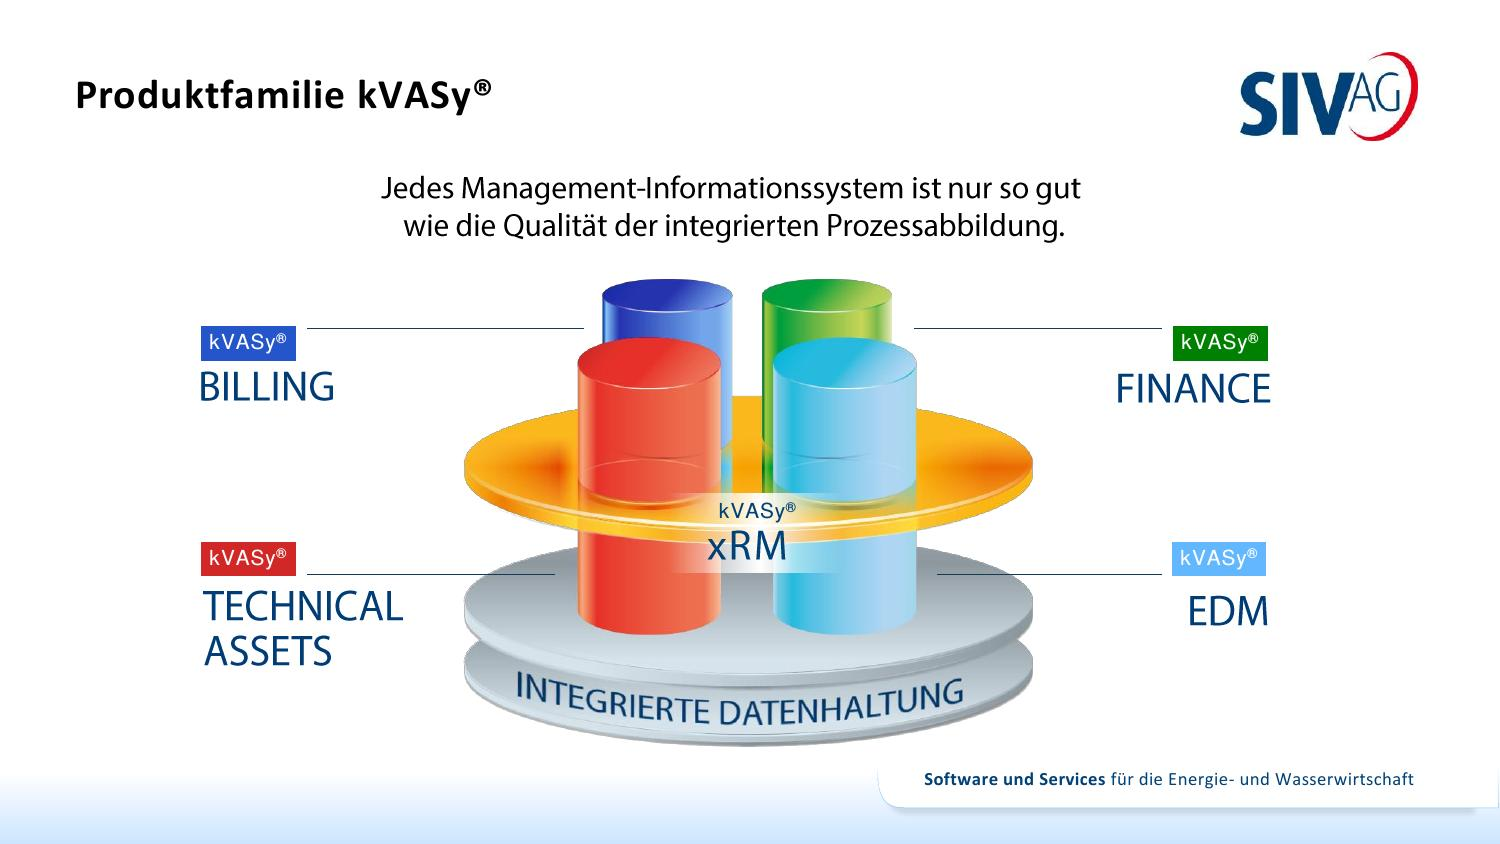
\includegraphics[scale=0.3]{bilder/kVASy_Schema.jpg}
% 		\caption{Ein Standard-Regelkreis}
% 		\label{pic:grund:regelkreis}
% 	\end{center}
% \end{figure}

% \subsection{Tabellen}
% Beispiel für eine Tabelle in \LaTeX{}
% \begin{table}[ht]
% 	\begin{center}
% 		\caption{Verwendete Matrizen}
% 		\begin{tabular}{|l|l|l|}
% 			\hline
% 			Matrix& Dimension& Symbol\\
% 			\hline
% 			Systemmatrix& $n\times n$& \textrm{A}\\
% 			\hline
% 			Ausgangsmatrix& $m\times n$& \textrm{C}\\
% 			\hline
% 		\end{tabular}
% 		\label{tab:grund:matrizen}
% 	\end{center}
% \end{table}
% 
% \subsection{Formeln}
% Beispiel für eine Formel in \LaTeX{}
% \begin{equation}
% 	c^2 = a^2 + b^2
% \end{equation}
% und noch eine Formel
% \begin{equation}
% 	f_1(x) = x_1 + x_2 + x_3
% \end{equation}
% Für weitere Möglichkeiten Formeln in \LaTeX{} einzufügen, schauen sie bitte in \cite{Peters2005}.
% 
% \subsection{{Bib\TeX}}
% Bib\TeX{} ermöglicht das erstellen eines Literaturverzeichnisses. Für die die sich weiter einarbeiten wollen, empfehle ich folgende Seite \cite{wiki:bibtex}.
% 
% \subsection{Abkürzungen}
% Es wird das Package \textit{glossary} verwendet. Mit ihm ist es möglich ein Abkürzungsverzeichnis und ein Glossary zu erstellen. Beispiel: \acrfull{lan} \acrfull{www}
